\documentclass{article}
\usepackage[utf8]{inputenc}
\usepackage{graphicx}
\usepackage{float}

\begin{document}
\title{Hands-on 16.05.2018 of the Computer Vision course at the
  University of Helsinki in May 2018}

\author{\emph{Vladimir Dobrodeev, student number 014690820}}
\maketitle

\newpage

\section{Hands-on}

\subsection{General information}

For this evaluation three images were used. First, there was \textit{bear.pbm}. Then, there were two self-made bmp images \textit{start.bmp} and \textit{car.bmp}.

\begin{figure}[H]
\centering
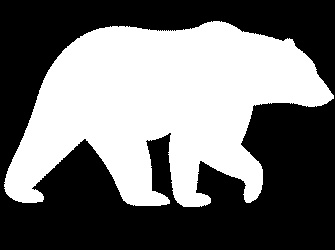
\includegraphics[width=\textwidth]{Bear}
\caption{Bear picture}
\end{figure}

\begin{figure}[H]
\centering
\includegraphics[width=\textwidth]{Star}
\caption{Star picture}
\end{figure}

\begin{figure}[H]
\centering
\includegraphics[width=\textwidth]{Car}
\caption{Car picture}
\end{figure}

\subsection{Distance transform}

The first to test was method \textit{distanceTransform}. This method calculates a distance in binary image between a non-zero pixel and closest zero pixel. As parameters it takes: \textit{src} - original binary image, \textit{distanceType} - show how to calculate the distance and \textit{maskSize} - size of the mask. Available distance types are:

\begin{itemize}
\item DIST_C: $max\left(|x_1 - x_2|, |y_1 - y_2|\right)$;
\item DIST_L1: $|x_1 - x_2| + |y_1 - y_2|$;
\item DIST_L2: $\sqrt{\left(x_1 - x_2\right)^2 + \left(y_1 - y_2\right)^2}$ (euclidian);
\item DIST_L12: $\sqrt{\left(x_1 - x_2\right)^2 + \left(y_1 - y_2\right)^2}$;
\end{itemize} 

\sec

\end{document}
%  LocalWords:  Jorma Laaksonen pdf py tex OpenCV libopencv dev jpg
%  LocalWords:  highgui imgproc imgcodecs greyscale png opencv ing
%  LocalWords:  texlive includegraphics Exactum Gür Ersalan
